\documentclass[12pt,a4paper]{article}
\usepackage[top=2cm,left=1cm,right=1cm,bottom=2cm]{geometry}
\usepackage{tikz}
 \usepackage[tikz]{bclogo}%
 \usetikzlibrary{calc,intersections}
\usetikzlibrary{arrows.meta}
\usetikzlibrary{decorations.pathmorphing}
\usepackage{amssymb,mathtools,amsthm}
\usepackage{fourier}
\usepackage{tkz-tab}
\usepackage{xcolor}
\usepackage{multicol, array, fancyhdr}
\usepackage{tasks}
\newcommand{\Lim}{\displaystyle\lim}
\renewcommand{\columnseprule}{1pt}
\renewcommand{\arraystretch}{1.5}
% \renewcommand{\displaystyle\frac}[2]{\displaystyle\displaystyle\frac{#1}{#2}}


%======================================================
\newtheoremstyle{mystyle}
  {\topsep}% espace avant
  {\topsep}% espace après
  {\upshape}% police du corps du théorème
  {}% indentation (vide pour rien, \parindent)
  {\bfseries\sffamily}% police du titre du théorème
  { :}% ponctuation après le théorème
  { }% après le titre du théorème (espace ou \newline)
  {%
    \rule[0.5\baselineskip]{0.5\textwidth}{1pt}%
    \newline\fcolorbox{black}{white}{%
      \thmname{#1}\thmnumber{ \textup{#2}}\thmnote{ \textnormal{(#3)}}%
    }%
    
    % \vspace{0.5em} % Adjust vertical space after the title
  }% spécifications du titre

\theoremstyle{mystyle}
\newtheorem{exo}{Exercice}

%======================================================



\begin{document}


\pagestyle{fancy}
\fancyhf{} % clear all header and footer fields
\fancyhead[L]{Lycée : Zitoun \hspace{1.5cm} Année scolaire : 2024-2025} % Left header
\fancyhead[C]{ \hspace{4cm} Niveau : 2BAC PC} % Right-Center header
\fancyhead[R]{Prof. Othmane Laksoumi} % Right header
\fancyfoot[C]{\thepage} % Footer


\begin{center}
    \textbf{\Large Dérivation et étude de fonctions numériques}
\end{center}
\begin{multicols*}{2}

\begin{exo}
Étudier la dérivabilité de la fonction $f$ en $a$ dans les cas suivants :
\begin{enumerate}
	\item $f(x) = 5x + 1$ et $a = 1$
	\item $f(x) = \sqrt{4x - 5}$ et $a = 2$
	\item $f(x) = x^3$ et $a = -2$
	\item $\begin{cases}
		f(x) = 1 - \cos(x) \text{ si } x\geq 0 \\
		f(x) = \sin(x) \text{ si } x < 0
	\end{cases}	
	$ et $a = 0$
\end{enumerate}
\end{exo}

\begin{exo}
On considère la fonction $f$ définie sur $\mathbb{R}$ par : $$f(x) = (1+x)^3$$
Donner l'approximation affine de $f$ au voisinage de $0$ et en déduire une valeur approchée du nombre\\ $b = (1,0004)^3$.
\end{exo}

\begin{exo}
Préciser l'ensemble sur lequel la fonction $f$ est dérivable et calculer $f^{\prime}$ lorqu'il existe dans chacun des cas suivants :
\begin{enumerate}
	\item $f(x) = x^3 - 5x^2 +\sqrt{5}x + \dfrac{1}{\sqrt{2}}$
	\item $f(x) = \sqrt{x^4 + x^2 + 1}$	
	\item $f(x) = \dfrac{2x + 1}{x^2 + x - 2}$
	\item $f(x) = x^4\sqrt{x} + \dfrac{1}{\sqrt{x}}$
	\item $f(x)  = \dfrac{3\sin(x) - 1}{\sin(x) - 1}$
	\item $f(x) = \left(\dfrac{x + 1}{x^2 + 3x + 1}\right)^2$
	\item $f(x) = x^3 - \sqrt{x}\tan(x) + \dfrac{\sin(x)}{x}$
	\item $f(x) = \cos\left(\sqrt{\dfrac{2x}{1+x^2}}\right)$

\end{enumerate}
\end{exo}

\begin{exo}
Soit $f$ la fonction définie sur $[-1;+\infty[$ par : $f(x) = \sqrt[3]{1+x}$.
\begin{enumerate}
	\item Montrer que $f$ est dérivable en $0$.
	\item En déduire l'pproximation affine de la fonction $f$ au voisinage de $0$.
	\item Déterminer des valeurs approchées des nombres : $\sqrt[3]{0,991}$ et $\sqrt[3]{1,007}$.
\end{enumerate}


\end{exo}

\begin{exo}
Calculer les limites suivantes :
$$\Lim_{x\to 3}\dfrac{(x-2)^{1986} - 1}{x - 3} \hspace{3mm} ; \hspace{3mm} \Lim_{x\to 2}\dfrac{x\sqrt{x+7} - 6}{x - 2} \hspace{3mm} ; \hspace{3mm} \Lim_{x\to 0}\dfrac{\sin(x)}{x}$$ 

$$\Lim_{x\to -1}\dfrac{\dfrac{1}{x+2} - 1}{x + 1} \hspace{1mm} ; \hspace{1mm} \Lim_{x\to \frac{\pi}{3}}\dfrac{2\cos(x) - 1}{\tan(x) - \sqrt{3}} \hspace{1mm} ; \hspace{1mm} \Lim_{x\to 1}\dfrac{x^4\sqrt{x} + \dfrac{1}{\sqrt{x}} - 2}{\sqrt{x} - 1}$$
\end{exo}

\begin{exo}

Dresser le tableau de variations de la fonction $f$ dans les cas suivants :
$$f(x) = x - \dfrac{1}{x} \ \ ; \ \ f(x) = 3x^4 - 2x^2 + 1 \ \ ; \ \ f(x) = \dfrac{4}{x^2 - 2x}$$
$$f(x) = \dfrac{x^2 + 4x + 1}{x + 1}$$
\end{exo}

\begin{exo}
	Dans la figure ci-après $(\mathcal{C}_f)$ est la courbe représentative d'une fonction $f$ dans le repére orthonormé $(O;\overrightarrow{i};\overrightarrow{j})$.
	\begin{center}
		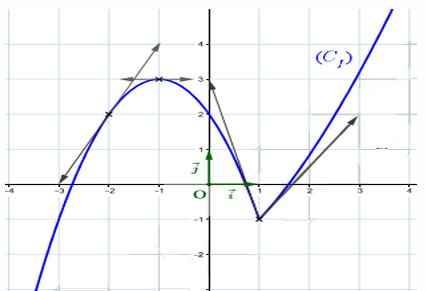
\includegraphics{graphe2.png}
	\end{center}
	\begin{enumerate}
		\item Déterminer graphiquement $f(-2)$, $f^{\prime}(-2)$ et $f^{\prime}(-1)$.
		\item Déterminer graphiquement $f^{\prime}_d(1)$ et $f^{\prime}_g(1)$.
		\item En déduire que $f$ n'est pas dérivable en $1$.
		\item Dresser le tableau de variations de $f$ sur $[-3;3]$ (on donne $f(3) = \dfrac{25}{8} $ ).
		\item En déduire le tableau de signe de $f^{\prime}$ sur $[-3;3]$.
		\end{enumerate}	
\end{exo}

\columnbreak

\begin{exo}
Soit $f$ la fonction définie sur $\mathbb{R}$ par $f(x) = x^3 + x + 1$.
	\begin{enumerate}
		\item Montrer que $f$ admet une fonction réciproque $f^{-1}$ définie sur $J$ à déterminer.
		\item Montrer que $f^{-1}$ est dérivable sur $J$.
		\item Calculer $f(1)$ et $f(-2)$. En déduire $\left(f^{-1}\right)^{\prime}(3)$ et $\left(f^{-1}\right)^{\prime}(-9)$
	\end{enumerate}
\end{exo}



\begin{exo}
	Soit $f$ la fonction définie sur $\left]-\dfrac{\pi}{2};\dfrac{\pi}{2}\right[$ par $f(x) = \tan(x)$
	\begin{enumerate}
		\item Montrer que $f$ admet une fonction réciproque $f^{-1}$ définie sur $J$ à déterminer.
		\item Déterminer l'ensemble de dérivabilité de $f^{-1}$.
		\item Montrer que : $(\forall x\in\mathbb{R})$; $\left(f^{-1}\right)^{\prime}(x) = \dfrac{1}{1 + x^2}$.
	\end{enumerate}
\end{exo}



\begin{exo}
Soit $g$ la fonction définie sur $\mathbb{R}$ par $$g(x) = x^5 + x^3 + x + 1$$
	\begin{enumerate}
		\item Etudier les variations de $g$.
		\item Montrer que l'équation $g(x) = 0$ admet une \\ solution unique $\alpha$ dans $\mathbb{R}$ et $-1 < \alpha < 0$.
		\item Donner le tableau de sign de $g$.	
	\end{enumerate}
	Soit $f$ la fonction définie sur $\mathbb{R}$ par :\\
		 $$f(x) = \dfrac{x^6}{6} + \dfrac{x^4}{4} + \dfrac{x^2}{2} + x$$
	\begin{enumerate}
		\item[4.] Calculer $f^{\prime}(x)$ pour tout $x\in\mathbb{R}$.
		\item[5.] En déduire les variations de $f$.
		\item[6.] Écrire une équation de la tangente à $(\mathcal{C}_f)$ au point d'abscisse $0$.
	\end{enumerate}
\end{exo}

\begin{exo}

Soit $f$ la fonction numérique définie par : $$f(x) = x - 1 + \sqrt{x - 1}$$

\begin{enumerate}
    \item Vérifier que : $D_f = [1; +\infty[$, puis calculer $\Lim_{x \to +\infty} f(x)$.
    \item Déterminer la branche infinie de $(\mathcal{C}_f)$ au \\voisinage de $+\infty$.
    \item Étudier la position relative de $(\mathcal{C}_f)$ et la première bissectrice du repère.
    \item Étudier la dérivabilité de $f$ à droite en 1, puis interpréter le résultat graphiquement.
    \item 
    \begin{enumerate}
        \item Montrer que $$(\forall x \in D_f-\{1\}); \ f'(x) = \frac{2\sqrt{x-1}+1}{\sqrt{x-1}}$$
        \item En déduire les variations de $f$.
    \end{enumerate}
    \item Montrer que $(\mathcal{C}_f)$ coupe la première bissectrice du repère en un unique point à déterminer.
    \item Tracer $(\mathcal{C}_f)$ dans un repère orthonormé.
    \item Montrer que $f$ admet une fonction réciproque $f^{-1}$ définie sur $J$ à déterminer.
    \item Tracer avec une autre couleur et dans le même repère précédent $(\mathcal{C}_{f^{-1}})$.
\end{enumerate}
\end{exo}

\begin{exo}

Soit $f$ la fonction numérique définie par : $f(x) = \dfrac{x}{\sqrt{x}-1}$.

\begin{enumerate}
    \item Vérifier que : $D_f = [0,1[ \cup ]1,+\infty[$, puis calculer les limites de $f$ aux bornes de $D_f$.
    \item Déterminer les deux branches infinies de $(\mathcal{C}_f)$.
    \item Étudier la dérivabilité de $f$ à droite en 0, puis interpréter le résultat graphiquement.
    \item 
    \begin{enumerate}
        \item Montrer que $\forall x \in D_f - \{0\}$, $f'(x) = \frac{\sqrt{x}-2}{2(\sqrt{x}-1)^2}$.
        \item Dresser le tableau de variations de $f$.
    \end{enumerate}
    	\item Étudier la concavité de $f$.
   \item Tracer $(\mathcal{C}_f)$ dans un repère orthonormé.\\
   Soit $g$ la restriction de la fonction $f$ sur l'intevalle $[0;1[$.
   \item Montrer que $g$ admet une fonction réciproque définie sur un intervalle $J$ à déterminer.
    \item Tracer avec une autre couleur et dans le même repère précédent $(\mathcal{C}_{g^{-1}})$.
\end{enumerate}

\end{exo}


\begin{exo}

Soit $f$ la fonction numérique définie sur $[1,+\infty[$ par : $f(x) = x \sqrt{x-1}$.

\begin{enumerate}
    \item Calculer $\Lim_{x \to +\infty} f(x)$.
    \item Étudier la continuité de $f$ sur $[1,+\infty[$.
    \item Déterminer la branche infinie de $(\mathcal{C}_f)$ au \\ voisinage de $+\infty$.
    \item Étudier la dérivabilité de $f$ à droite en 1, puis interpréter le résultat graphiquement.
    \item 
    \begin{enumerate}
        \item Montrer que $$(\forall x \in ]1,+\infty[); \ f'(x) = \frac{3x-2}{2\sqrt{x-1}}$$
        \item En déduire les variations de $f$.
    \end{enumerate}
    \item 
    \begin{enumerate}
        \item Montrer que $$(\forall x \in ]1,+\infty[); \ f''(x) = \frac{3x-4}{4\sqrt{(x-1)^3}}$$
        \item En déduire que $(\mathcal{C}_f)$ admet un point d’inflexion $A$ dont on déterminera ses coordonnées.
    \end{enumerate}
    \item Étudier la position relative de $(\mathcal{C}_f)$ et la \\première bissectrice du repère.
    \item Tracer $(\mathcal{C}_f)$ dans un repère orthonormé.
    \item 
    		\begin{enumerate}
    			\item Montrer que $f$ admet une fonction réciproque $f^{-1}$ définie sur un intervalle $J$ à déterminer.
    			\item Montrer que $f^{-1}$ est dérivable en $2$, puis déterminer $\left(f^{-1}\right)^{\prime}(2)$.
    		\end{enumerate}
    	\item Tracer avec une autre couleur et dans le même repère précédent $(\mathcal{C}_{f^{-1}})$.
\end{enumerate}

\end{exo}



%\begin{exo}
%\text{ }
%\\
%\underline{\textbf{Partie A : }}\\
%Soit $u$ la fonction numérique définie sur $\mathbb{R}$ par : $u(x) = 7x^3 + 6x + 1$.
%
%\begin{enumerate}
%    \item Déterminer $u'(x)$, pour tout $x$ de $\mathbb{R}$.
%    \item Dresser le tableau de variations de $u$.
%    \item En déduire que : $\forall x \in [0, +\infty[$, $u(x) > 0$.
%\end{enumerate}
%\underline{\textbf{Partie B : }}\\
%Soit $f$ la fonction numérique définie sur $[0, +\infty[$ par : $f(x) = (x^3 + 2x + 1)\sqrt{x} - 3$.
%
%\begin{enumerate}
%    \item Montrer que : $\Lim_{x \to +\infty} f(x) = +\infty$, puis déterminer la branche infinie de $f$ au voisinage de $+\infty$.
%    \item Montrer que $f$ est continue sur $[0, +\infty[$.
%    \item Étudier la dérivabilité de $f$ à droite en $0$, puis interpréter le résultat graphiquement.
%    \item 
%    \begin{enumerate}
%        \item Montrer que : $\forall x \in ]0, +\infty[$, $f'(x) = \frac{u(x)}{2\sqrt{x}}$.
%        \item En utilisant la question A.3), déduire que $f$ est strictement croissante sur $[0, +\infty[$.
%    \end{enumerate}
%    \item Montrer que $(\mathcal{C}_f)$ coupe l'axe des abscisses en un seul point d'abscisse $\alpha$, puis vérifier que : $0,8 < \alpha < 0,9$.
%    \item Déterminer l'équation de la tangente $(T)$ à la courbe $(\mathcal{C}_f)$ représentant la fonction $f$ au point d'abscisse 1.
%    \item Tracer $(T)$ et $(\mathcal{C}_f)$ dans un repère orthonormé (on admet que $(\mathcal{C}_f)$ possède un point d’inflexion d’abscisse $\beta \approx 0,1 \; \text{« unité : 2cm »}$).
%    \item 
%    \begin{enumerate}
%        \item Montrer que $f$ admet une fonction réciproque $f^{-1}$ définie sur un intervalle $J$ à déterminer.
%        \item Tracer dans le même repère précité la courbe $(\mathcal{C}_{f^{-1}})$.
%    \end{enumerate}
%\end{enumerate}
%
%\end{exo}

\begin{exo}
\text{ }
\underline{\textbf{Partie A : }}\\
Soit $u$ la fonction numérique définie sur $\mathbb{R}^*_+$ par :
$$u(x) = 3 - \dfrac{2}{\sqrt{x}} - \dfrac{1}{x^2}$$
\begin{enumerate}
	\item Calculer $u^{\prime}(x)$ pour tout $x\in\mathbb{R}^*_+$.
	\item En déduire que $u$ est strictement croissante sur $\mathbb{R}^*_+$.
	\item 
		\begin{enumerate}
			\item Calculer $u(1)$.
			\item En déduire que $u(x)\geq 0$ pour tout\\ $x\in[1;+\infty[$ et que $u(x) \leq 0$ pour tout\\ $x\in]0;1]$.
		\end{enumerate}
\end{enumerate}

\underline{\textbf{Partie B : }}\\
Soit $f$ la fonction définie sur $\mathbb{R}^*_+$ par :
\[
f(x) = 4 \sqrt{x} - 3x - \frac{1}{x}
\]
et soit $\mathcal{C}_f$, sa courbe représentative dans un repère orthonormé $(O; \vec{i}; \vec{j})$.

\begin{enumerate}
    \item[a)] Calculer les limites : $\Lim_{x \to 0^+} f(x)$ et $\Lim_{x \to +\infty} f(x)$.
    \item[b)] Étudier les branches infinies de la courbe $\mathcal{C}_f$.
    
    \item[2)] 
    \begin{enumerate}
        \item[a)] Justifier la dérivabilité de $f$ sur $\mathbb{R}^*_+$ puis montrer que :
        \[
        (\forall x \in \mathbb{R}^*_+) \ f'(x) = -u(x)
        \]
        \item[b)] Étudier le signe de $f'(x)$ puis dresser le tableau de variations de la fonction $f$.
    \end{enumerate}
    
    \item[3)] 
    \begin{enumerate}
        \item[a)] Calculer $f'(x)$ pour tout $x \in D_f$.
        \item[b)] Étudier le signe de $f'(x)$ puis dresser le tableau de variations de la fonction $f$.
        \item[c)] En déduire que :
        \[
        (\forall x \in \mathbb{R}^*_+) \ 4\sqrt{x} \leq 3x + \frac{1}{x}
        \]
    \end{enumerate}
    
    \item[4)] Construire la courbe $\mathcal{C}_f$.
 
\end{enumerate}

\end{exo}

\begin{exo}
\text{ }\\
\underline{\textbf{Partie A : }}\\
Soit $g$ la fonction numérique sur $\mathbb{R}$ par : $g(x) = x^3 - x^2 + 3x + 1$.

\begin{enumerate}
    \item Calculer les limites de $g$ en $+\infty$ et en $-\infty$.
    \item Étudier les variations de $g$ sur $\mathbb{R}$.
    \item Montrer que l’équation $g(x) = 0$ admet une seule solution $\alpha$ sur $\mathbb{R}$, et que : $-1 < \alpha < 0$.
    \item Déterminer le signe de $g(x)$ suivant les valeurs de $x$.
\end{enumerate}

\underline{\textbf{Partie B : }}\\
Soit $f$ la fonction numérique définie par : $$f(x) = x - \frac{2}{x^2 + 1}$$

\begin{enumerate}
    \item Déterminer $D_f$, puis calculer les limites de $f$ en $+\infty$ et en $-\infty$.
    \item Étudier la continuité de $f$ sur $D_f$.
    \item Montrer que : $\forall x \in D_f$, $f'(x) = \dfrac{(x+1)g(x)}{(x^2 + 1)^2}$.
    \item Étudier les variations de $f$, puis dresser son tableau de variations.
    \item Vérifier que la première bissectrice du repère est l’asymptote oblique de $(\mathcal{C}_f)$ au voisinage de $-\infty$ et de $+\infty$.
    \item Étudier la position relative de $(\mathcal{C}_f)$ et la première bissectrice du repère.
    \item Soit $h$ la restriction de $f$ sur l’intervalle $I = [0,+\infty[$.
    \begin{enumerate}
        \item Montrer que $h$ admet une fonction réciproque $h^{-1}$ définie sur un intervalle $J$ à déterminer.
        \item Dresser le tableau de variations de $h^{-1}$.
    \end{enumerate}
\end{enumerate}
\end{exo}




\begin{exo}

Soit $f$ la fonction numérique définie par :
$
f(x) = x - 1 - \sqrt{\dfrac{x}{x-1}}
$
et soit $\mathcal{C}_f$, sa courbe représentative dans un repère orthonormé $(O; \vec{i}; \vec{j})$.

\begin{enumerate}
    \item Vérifier que : $D_f = ] - \infty ; 0 ] \cup ] 1 ; + \infty [$.
    \item Calculer $\Lim_{x \to + \infty} f(x)$ et interpréter le résultat obtenu.
    \item 
    \begin{enumerate}
        \item Montrer que la droite $(D) : y = x - 2$ est une asymptote oblique de $\mathcal{C}_f$ au voisinage de $+ \infty$ et $- \infty$.
        \item Étudier la position relative de la courbe $\mathcal{C}_f$ par rapport à la droite $(D)$.
    \end{enumerate}
    \item Étudier la dérivabilité à gauche en $0$ de la fonction $f$, puis interpréter graphiquement le résultat obtenu.
    \item 
    \begin{enumerate}
        \item Calculer $f'(x)$ pour tout $x \in D_f - \{ 0 \}$.
        \item Étudier le signe de $f'(x)$ puis dresser le tableau de variations de la fonction $f$.
    \end{enumerate}
    \item Écrire l'équation de la tangente $(T)$ à la courbe $\mathcal{C}_f$ au point d'abscisse 2.
    
    \item 
    \begin{enumerate}
        \item Montrer que la courbe $\mathcal{C}_f$ coupe l'axe des abscisses en un unique point et dont l'abscisse $\alpha$ appartient à l'intervalle $\left] 2 ; \dfrac{5}{2} \right[$.
        \item Montrer que : $\alpha - \sqrt[3]{\alpha} = 1$.
    \end{enumerate}
    \item Construire la courbe $\mathcal{C}_f$.
    \item Soit $g$ la restriction de la fonction $f$ sur $]1 ; + \infty[$.
    \begin{enumerate}
        \item Montrer que $g$ admet une fonction \\réciproque $g^{-1}$ définie sur un intervalle $J$ à déterminer.
        \item Montrer que $g^{-1}$ est dérivable sur $J$.
        \item Montrer que $(g^{-1})^{\prime}(0) = \dfrac{2(\alpha - 1)^3}{1 + 2(\alpha - 1)^3}$.
        \item Tracer la courbe $\mathcal{C}_{g^{-1}}$ dans le repère $(O;\vec{i};\vec{j})$.
    \end{enumerate}
\end{enumerate}

\end{exo}

\begin{exo}
Soit $f$ la fonction numérique définie sur $\mathbb{R}$ par :
\[
f(x) = \begin{cases} 
x - 1 + 2 \sqrt{1 - x} & \text{si } x < 1 \\
\dfrac{x^3 - 1}{x^3 + 1} & \text{si } x \geq 1
\end{cases}
\]

et soit $\mathcal{C}_f$ sa courbe représentative dans un repère orthonormé $(O; \overrightarrow{i}; \overrightarrow{j})$.

\begin{enumerate}
    \item Calculer $\lim\limits_{x \to -\infty} f(x)$ et $\lim\limits_{x \to +\infty} f(x)$.
    \item 
    \begin{enumerate}
        \item Montrer que la fonction $f$ est continue en $1$.
        \item Étudier la dérivabilité à gauche et à droite de la fonction $f$ en $1$ puis interpréter graphiquement les résultats obtenus.
    \end{enumerate}
    \item 
    \begin{enumerate}
        \item Montrer que la fonction $f$ est strictement croissante sur l'intervalle $]1; +\infty[$.
        \item Montrer que pour tout $x \in ]-\infty; 1[$ :
        \[
        f'(x) = \frac{-x}{\sqrt{1 - x} \left( 1 + \sqrt{1 - x} \right)}
        \]
        \item Dresser le tableau de variations de $f$.
     \end{enumerate}
    \item Étudier les branches infinies de la courbe $\mathcal{C}_f$.
    \item Tracer la courbe $\mathcal{C}_f$ dans le repère $(O; \overrightarrow{i}; \overrightarrow{j})$.
    \item Soit $g$ la restriction de la fonction $f$ sur $[1; +\infty[$.
    \begin{enumerate}
        \item Montrer que $g$ admet une fonction réciproque $g^{-1}$ définie sur un intervalle $J$ à déterminer.
        \item Calculer $g^{-1}(x)$ pour tout $x \in J$.
    \end{enumerate}
\end{enumerate}

\end{exo}


\end{multicols*}





\begin{exo}
Soit $f$ une fonction deux fois dérivables sur l'intervalle $[-6;5]$.\\
On donne dans le repère ci-dessous, la courbe $\mathcal{C}^{\prime}$, représentative de la fonction $f^{\prime}$, dérivée de $f$.
\begin{center}
	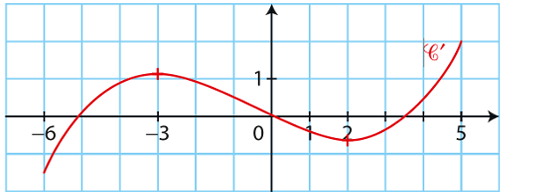
\includegraphics[scale=0.8]{graphe3.png}
\end{center}
\begin{enumerate}
	\item Dresser le tableau de variations de $f$ sur l'intervalle $[-6;5]$.
	\item Étudier la concavité de $f$ sur l'intervalle $[-6;5]$ et préciser les abscisses des points d'inflexion de la courbe $\mathcal{C}$ représentative de la fonction $f$.
\end{enumerate}

\end{exo}

\begin{exo}
La figure en-dessous représente les courbe représentative $\mathcal{C}_f$ et $\mathcal{C}_g$ des fonctions numériques $f$ et $g$ respectivement.
\begin{center}
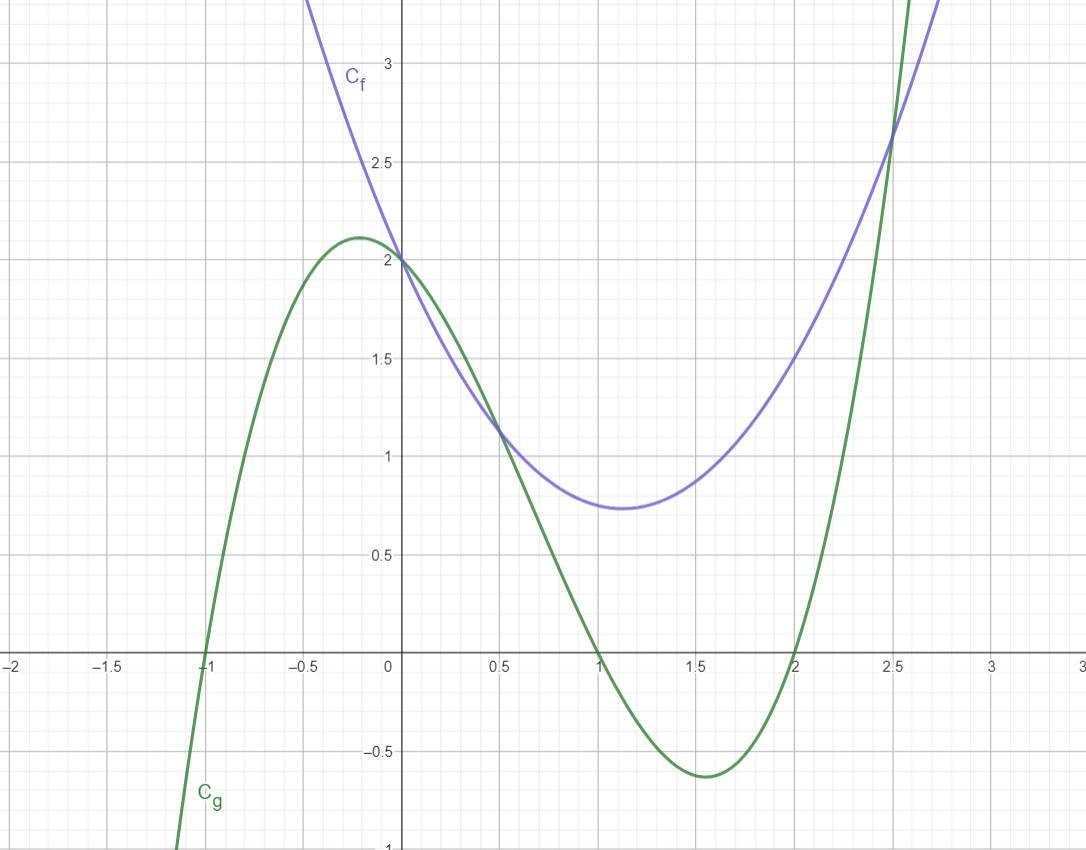
\includegraphics[scale=0.6]{graphe4.png}
\end{center}
\begin{enumerate}
	\item Résoudre graphiquement l'équation \\$g(x) =0$.
	\item Résoudre graphiquement les inéquation \\$g(x) \geq 0$ ; $g(x) \leq 0$ ; $f(x) > 0$ et $f(x) < 0$.
	\item Résoudre graphiquement l'équation \\$f(x) = g(x)$.
	\item Résoudre graphiquement les inéquation \\$f(x) \geq g(x)$ et $f(x) \leq g(x)$.
\end{enumerate}

\end{exo}



















\end{document}